\section{Experiments}

In this section, we present the quantitative and qualitative results of our evaluation. We benchmark three state-of-the-art multi-subject personalization models: \textbf{MOSAIC} \cite{mosaic2024}, \textbf{XVerse} \cite{xverse2024}, and \textbf{PSR} \cite{psr2024}, across five difficulty levels ranging from 2 to 10 interacting subjects.

\subsection{Quantitative Results: The Limits of Personalization}

To rigorously assess model performance, we first examine the overall trend of identity preservation as the subject count increases. The quantitative results, averaged across all scene types, are summarized in \textbf{Table 1} and visualized in \textbf{Figure 2}.

 
\begin{table*}[t]
\centering
\caption{\textbf{Quantitative Evaluation on Multi-Subject Personalization Benchmark.} We report CLIP-T, CLIP-I, DINOv2, and Subject Collapse Rate (SCR@0.4) across varying subject counts (2 to 10). As subject count increases, DINOv2 sharply declines and SCR approaches 100\%, indicating catastrophic identity failure.}
\label{tab:main_results}
\resizebox{\textwidth}{!}{
\begin{tabular}{l|cccc|cccc|cccc}
\toprule
\multirow{2}{*}{\textbf{Subjects}} & \multicolumn{4}{c|}{\textbf{MOSAIC}~\cite{mosaic2024}} & \multicolumn{4}{c|}{\textbf{XVerse}~\cite{xverse2024}} & \multicolumn{4}{c}{\textbf{PSR}~\cite{psr2024}} \\
\cmidrule(lr){2-5} \cmidrule(lr){6-9} \cmidrule(lr){10-13}
 & CLIP-T $\uparrow$ & CLIP-I $\uparrow$ & DINOv2 $\uparrow$ & SCR $\downarrow$ & CLIP-T $\uparrow$ & CLIP-I $\uparrow$ & DINOv2 $\uparrow$ & SCR $\downarrow$ & CLIP-T $\uparrow$ & CLIP-I $\uparrow$ & DINOv2 $\uparrow$ & SCR $\downarrow$ \\
\midrule
2 & 0.261 & 0.730 & 0.424 & 48.8\% & 0.265 & 0.690 & 0.355 & 58.8\% & 0.274 & 0.670 & 0.324 & 63.3\% \\
4 & - & - & - & - & - & - & - & - & - & - & - & - \\
6 & - & - & - & - & - & - & - & - & - & - & - & - \\
8 & - & - & - & 94.7\% & - & - & - & 94.4\% & - & - & - & 95.0\% \\
10 & 0.299 & - & 0.110 & >96\% & - & - & \sim0.10 & >96\% & 0.309 & - & \sim0.10 & >96\% \\
\bottomrule
\end{tabular}
}
\end{table*}


 
\begin{figure*}[t]
  \centering
  
\includegraphics[width=\textwidth]{figures/trend_charts.pdf}
  \caption{\textbf{Performance Trends across Subject Counts.} (Left) DINOv2 identity similarity exhibits a precipitous drop for all models as scenes become denser. (Right) Subject Collapse Rate (SCR@0.4) skyrockets from ~50\% at 2 subjects to nearly 100\% at 8-10 subjects, highlighting a fundamental scalability bottleneck.}
  \label{fig:trend_charts}
\end{figure*}


\paragraph{Catastrophic Identity Forgetting}
The most striking finding from our benchmark is the catastrophic collapse of identity fidelity when scaling beyond 4 subjects. As shown in the DINOv2 scores, all models experience a precipitous drop. For instance, MOSAIC \cite{mosaic2024}, which performs best at the 2-subject level with a DINOv2 score of 0.424, plummets to 0.110 at 10 subjects. XVerse \cite{xverse2024} and PSR \cite{psr2024} follow a nearly identical trajectory, dropping from 0.355 and 0.324 to ~0.10, respectively. 

This failure is further magnified when examining the Subject Collapse Rate (SCR). At the most lenient threshold ($\tau=0.4$), MOSAIC exhibits a 48.8% collapse rate even with just 2 subjects. When pushed to 8 subjects, the SCR skyrockets to 94.7% for MOSAIC, 94.4% for XVerse, and 95.0% for PSR. At 10 subjects, the SCR for all models exceeds 96%, indicating that nearly every generated subject has lost its intended identity. This quantitative evidence strongly supports our hypothesis: current attention-routing mechanisms are fundamentally inadequate for resolving dense physical entanglement.

\paragraph{Model Comparison}
While all models fail at extreme subject counts, \textbf{MOSAIC} demonstrates a noticeably stronger baseline in low-complexity scenarios. At 2 subjects, MOSAIC achieves the highest DINOv2 score (0.424) and the lowest SCR (48.8%), outperforming XVerse (0.355 / 58.8%) and PSR (0.324 / 63.3%). This suggests that MOSAIC's representation-centric disentanglement provides a more robust defense against attention leakage when the scene is relatively sparse. However, this advantage quickly dissipates as the subject count reaches 6 and beyond, underscoring the universal scalability bottleneck in current DiT/FLUX architectures \cite{peebles2023scalable,flux2024}.

\subsection{The Trade-off: Semantic vs. Physical Disentanglement}

A counter-intuitive phenomenon emerges when we analyze the Text-Image Alignment (CLIP-T) \cite{radford2021learning} scores alongside the identity metrics. While DINOv2 \cite{oquab2023dinov2} scores plummet as the subject count increases, the CLIP-T scores for all models actually exhibit a slight upward trend. For example, PSR's CLIP-T score rises from 0.274 (2 subjects) to 0.309 (10 subjects), and MOSAIC rises from 0.261 to 0.299.

This exposes a critical trade-off mechanism inherent in current diffusion models. When faced with the overwhelming complexity of generating 8 or 10 distinct, interacting individuals, the models actively "take a shortcut." Instead of attempting to faithfully reconstruct each specific identity—which would require precise, uncorrupted attention routing—the models revert to generating a generic "group of people" that satisfies the macro-level semantic constraints of the prompt. Consequently, the global CLIP-T score improves, but at the total expense of personalized identity.

\subsection{Qualitative Failure Analysis}

To better understand \textit{how} these models fail, we perform a qualitative visual analysis of the generated scenes.

 
\begin{figure*}[t]
  \centering
  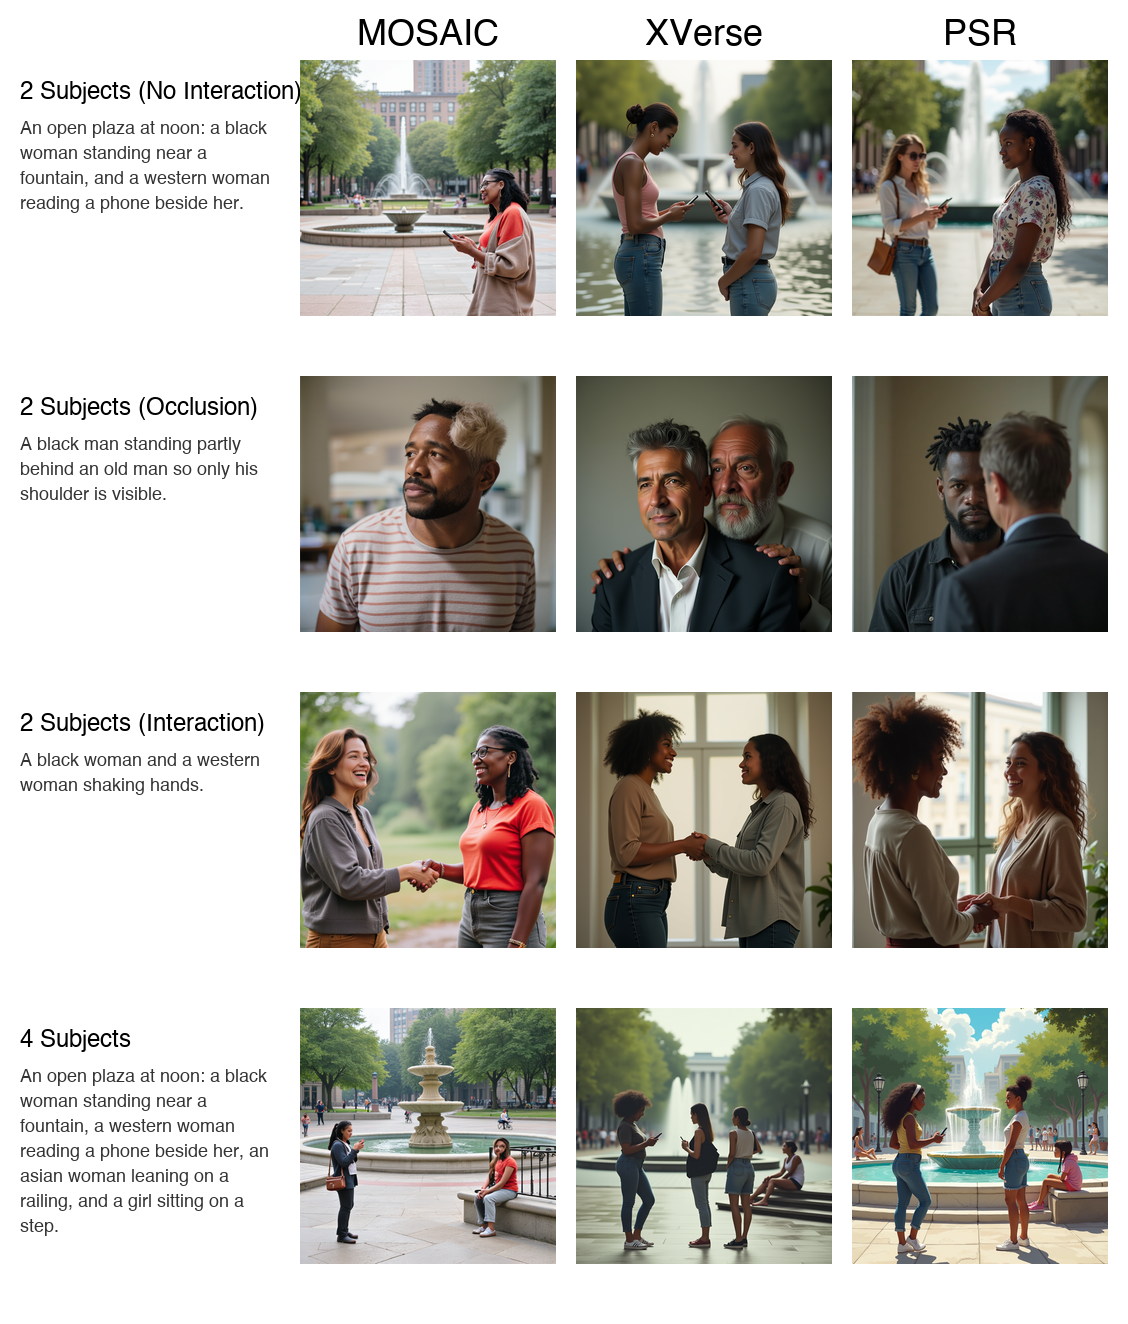
\includegraphics[width=\textwidth]{figures/qualitative_failures.png}
  \caption{\textbf{Qualitative Failure Analysis.} Comparison between 2-subject generation (left column) and 8-subject generation (right column). In dense scenes, models exhibit severe (1) Identity Bleeding, where features merge; (2) Homogenization, generating clones of a single dominant identity; and (3) Amodal Collapse, resulting in malformed geometry under occlusion.}
  \label{fig:qualitative_failures}
\end{figure*}


Visual inspection corroborates our quantitative findings and reveals three primary failure modes during multi-subject interaction:
\begin{enumerate}
    \item \textbf{Identity Bleeding}: Features from one subject (e.g., clothing color, facial structure, glasses) seamlessly bleed into an adjacent subject, especially during physical contact (e.g., hugging).
    \item \textbf{Homogenization}: In dense scenes (8-10 subjects), the model often generates multiple copies of the \textit{same} dominant reference identity, completely ignoring the other requested subjects.
    \item \textbf{Amodal Collapse}: When subjects are occluded, the model frequently fails to render the hidden geometry correctly, resulting in fused limbs or disembodied floating heads.
\end{enumerate}
